\section{OPTIMIST}

\begin{frame}{Problem Formulation}

\onslide<+->\begin{block}{Decision Set or Arms Set}
The parameter space $\Theta\subseteq\Reals^d$.
\end{block}

\onslide<+->\begin{block}{Procedure}
At every decision step $t\in[0,1,2,\dots,T]$:
	\begin{enumerate}
			\item<+-> \textbf{Select} an arm $\vtheta_t\in\Theta$;
			\item<+-> \textbf{Sample} a trajectory $\tau_t\in\Tau$ by following $\pi_{\vtheta_t}$;
			\item<+-> \textbf{Observe} the cumulative return $\Rew(\tau_t)$.
		\end{enumerate}
\end{block}

\onslide<+->\begin{block}{Goal}
\begin{itemize}
\item \textbf{Minimize} $Regret(T) = \sum_{t=0}^{T}\mu(\vtheta^*)-\mu(\vtheta_t)$, where $\vtheta^*=\arg\max_{\vtheta\in\Theta}\mu(\vtheta)$
\end{itemize}
\end{block}

%\onslide<+->\begin{block}{Goal}
%\begin{itemize}
%\item Maximize the total expected return $\sum_{t=0}^T \Exp_{\tau_t\sim p_{\vtheta_t}}[\Rew(\tau_t)] = \sum_{t=0}^T \mu(\vtheta)$
%\item<+-> Alternatively, minimize \textbf{regret}.
%\end{itemize}
%\end{block}

\end{frame}


\begin{frame}{Regret}

\onslide<+->\begin{block}{Decision Set or Arms Set}
The parameter space $\Theta\subseteq\Reals^d$.
\end{block}

\end{frame}

%	\onslide<2->{
%	\textbf{Rewards}: portfolio log-return with transaction costs
%		\begin{equation*}
%			R_{t+1} = \log \left\{ 1 + \sum^{I}_{i=0} \left[ 
%				\tikz[baseline]{
%		        	\node[anchor=base] (t1) {$a_t^i X_{t+1}^i$};
%		        } - 
%		        \tikz[baseline]{
%		        	\node[anchor=base] (t2) {$\delta_i \left| a_t^i - \widetilde{a}_t^i \right|$};
%		       	} -
%		       	\tikz[baseline]{
%		       		\node[anchor=base] (t3) {$\delta_s {(a_t^i)}^-$};
%		       	} \right] -
%		       	\tikz[baseline]{
%		       		\node[anchor=base] (t4) {$\delta_f \mathbf{1}_{{a}_t \neq \tilde{{a}}_{t-1}}$};
%		       	} \right\}	 	
%		 \end{equation*}
%	}
%	
%	\onslide<7->{
%	\textbf{Actions}: Portfolio weights
%		\begin{equation*}
%			\{a_t^i\}_{i=0}^I \;\;\; \text{s.t.}\;\;\; \sum^{I}_{i=0} a_t^i = 1 \;\;\;\;\; \forall t \in \{0, 1, 2, \ldots\}
%		\end{equation*}
%	}
%
%	\onslide<8->{
%	\textbf{States}: assets past returns and current allocation
%		\begin{equation*}
%			S_t = \{X, X_t, X_{t-1}, \ldots, X_{t-P}, \tilde{a}_t\}
%		\end{equation*}
%	}
%	
%	\onslide<3|handout:0>{
%		\begin{tikzpicture}[overlay]
%				\node[draw=SteelBlue, circle, line width=3pt, minimum size=2cm] at (t1) {};
%		\end{tikzpicture}
%	}
%	
%	\onslide<4|handout:0>{
%		\begin{tikzpicture}[overlay]
%				\node[draw=SteelBlue, circle, line width=3pt, minimum size=2cm] at (t2) {};
%		\end{tikzpicture}
%	}
%		
%	\onslide<5|handout:0>{
%		\begin{tikzpicture}[overlay]
%				\node[draw=SteelBlue, circle, line width=3pt, minimum size=2cm] at (t3) {};
%		\end{tikzpicture}
%	}
%			
%	\onslide<6|handout:0>{
%		\begin{tikzpicture}[overlay]
%				\node[draw=SteelBlue, circle, line width=3pt, minimum size=2cm] at (t4) (g) {};
%		\end{tikzpicture}
%	}
%\end{frame}
%
%\begin{frame}[c]{Synthetic Asset: Convergence}
%\begin{figure}[t!]
%	\centering
%	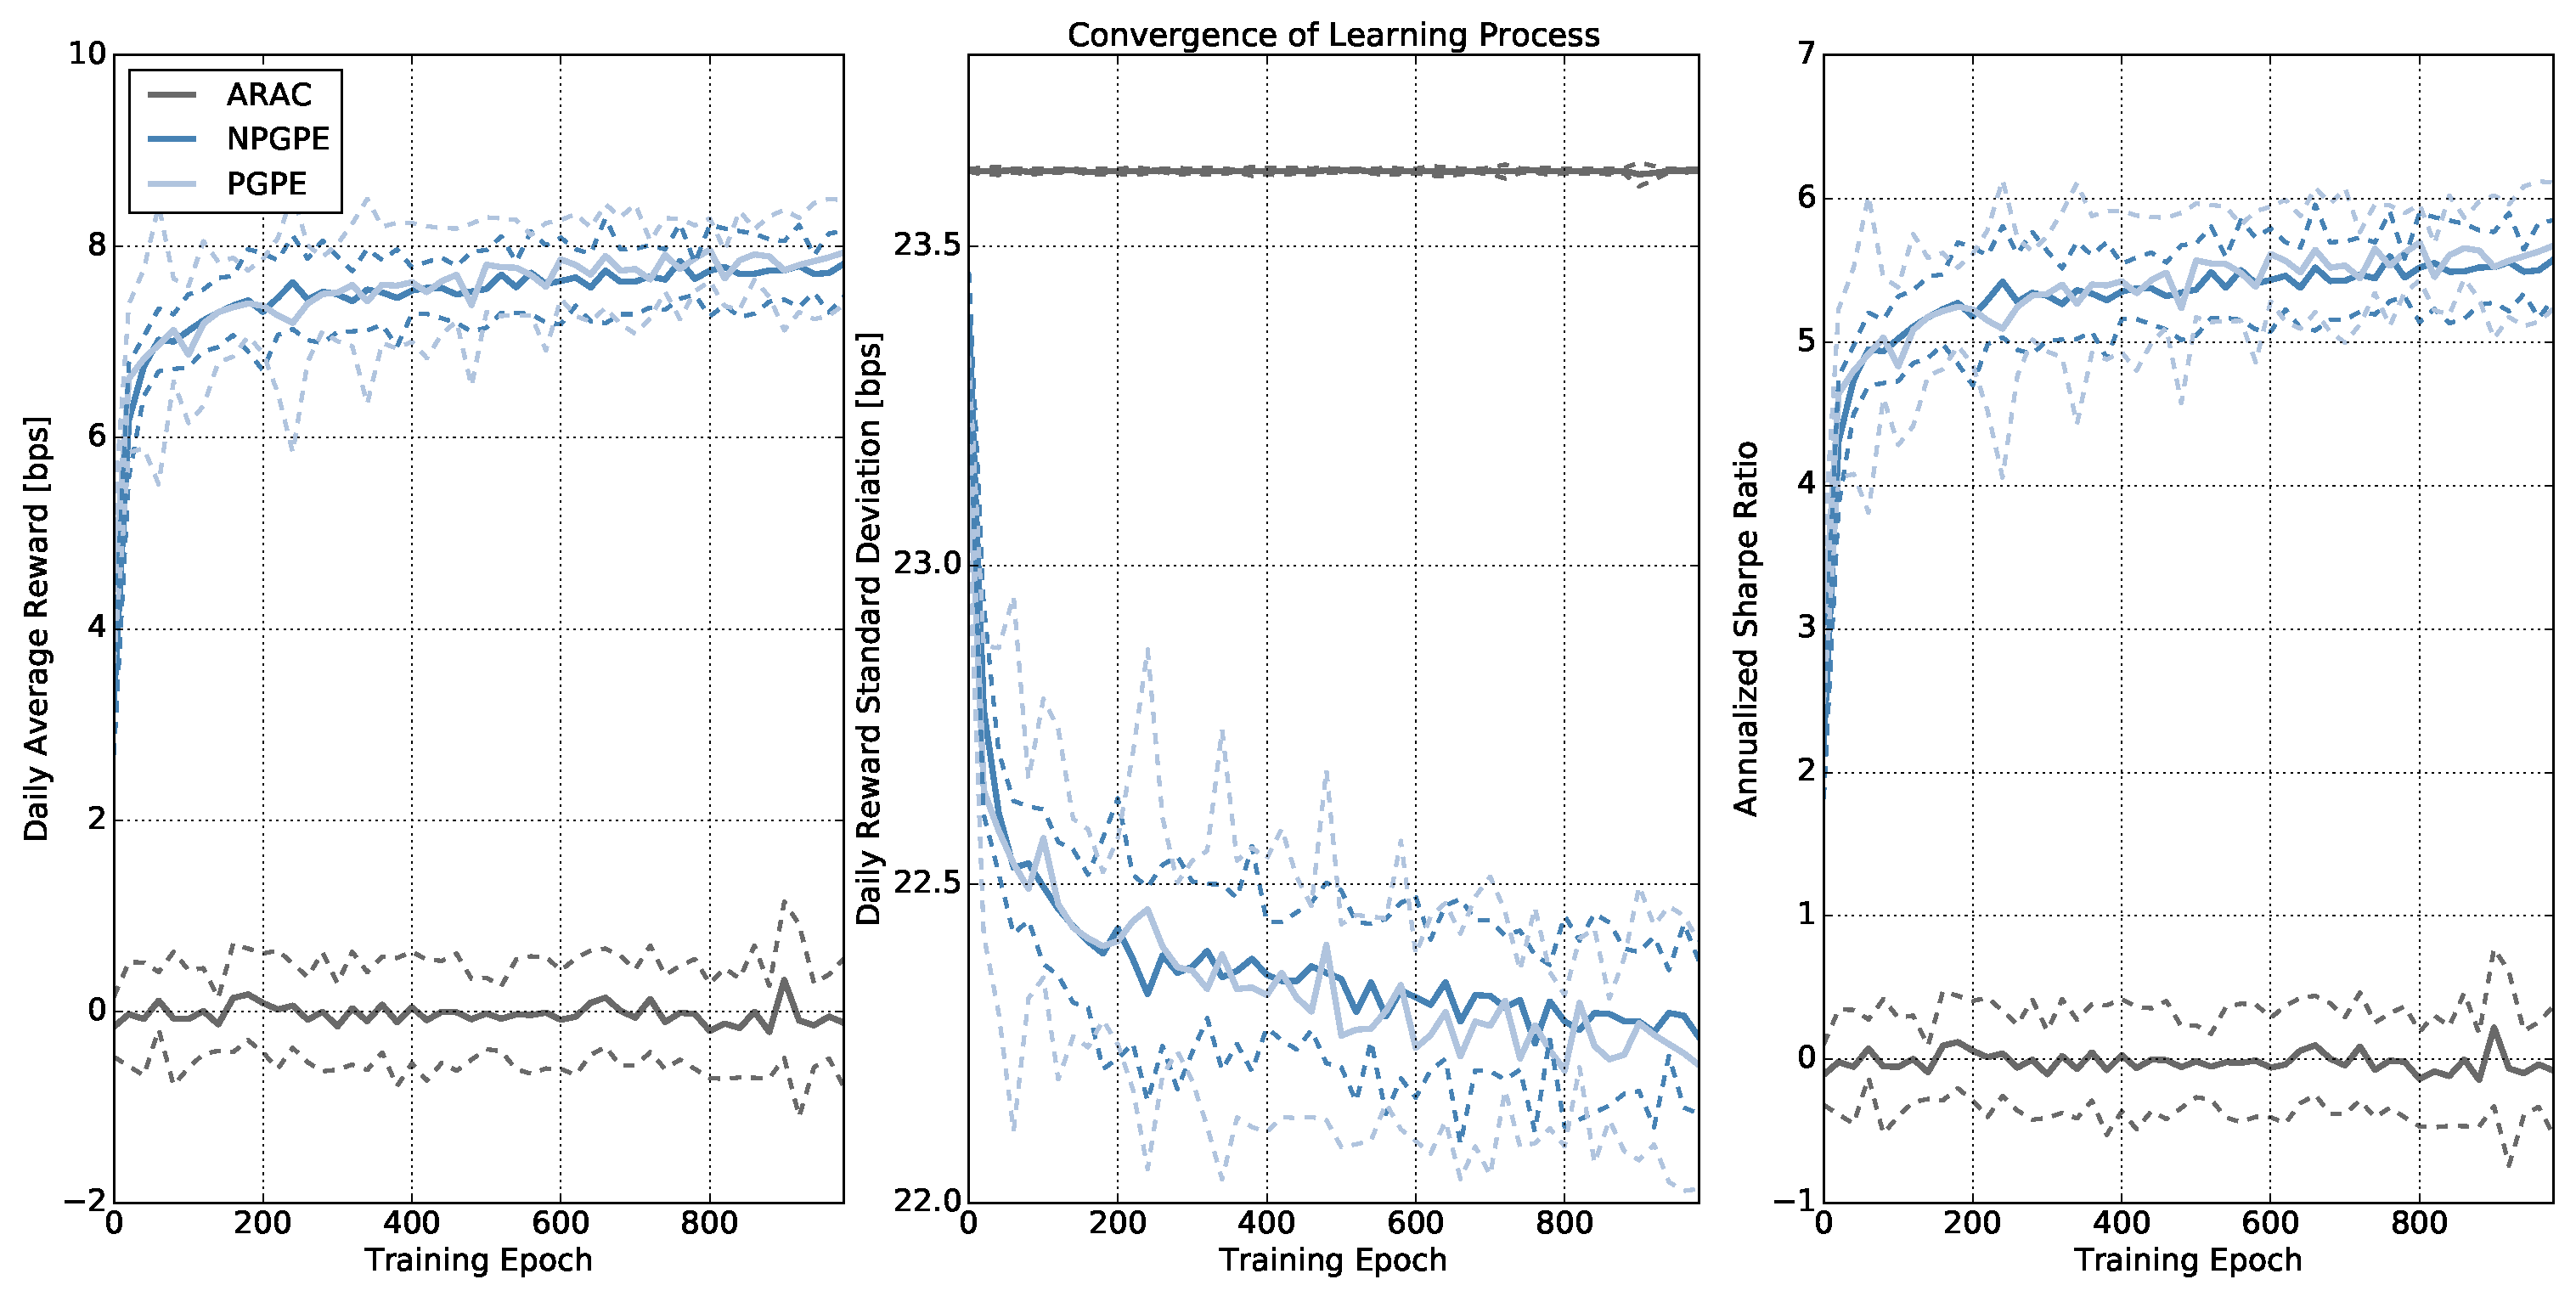
\includegraphics[height=5cm,width=0.8\textwidth]{Images/6_0_single_synthetic_neutral_convergence}
%\end{figure}
%\end{frame}
%
%
%\begin{frame}[c]{Synthetic Asset: Backtest Performance}
%\begin{figure}[t]
%	\centering
%	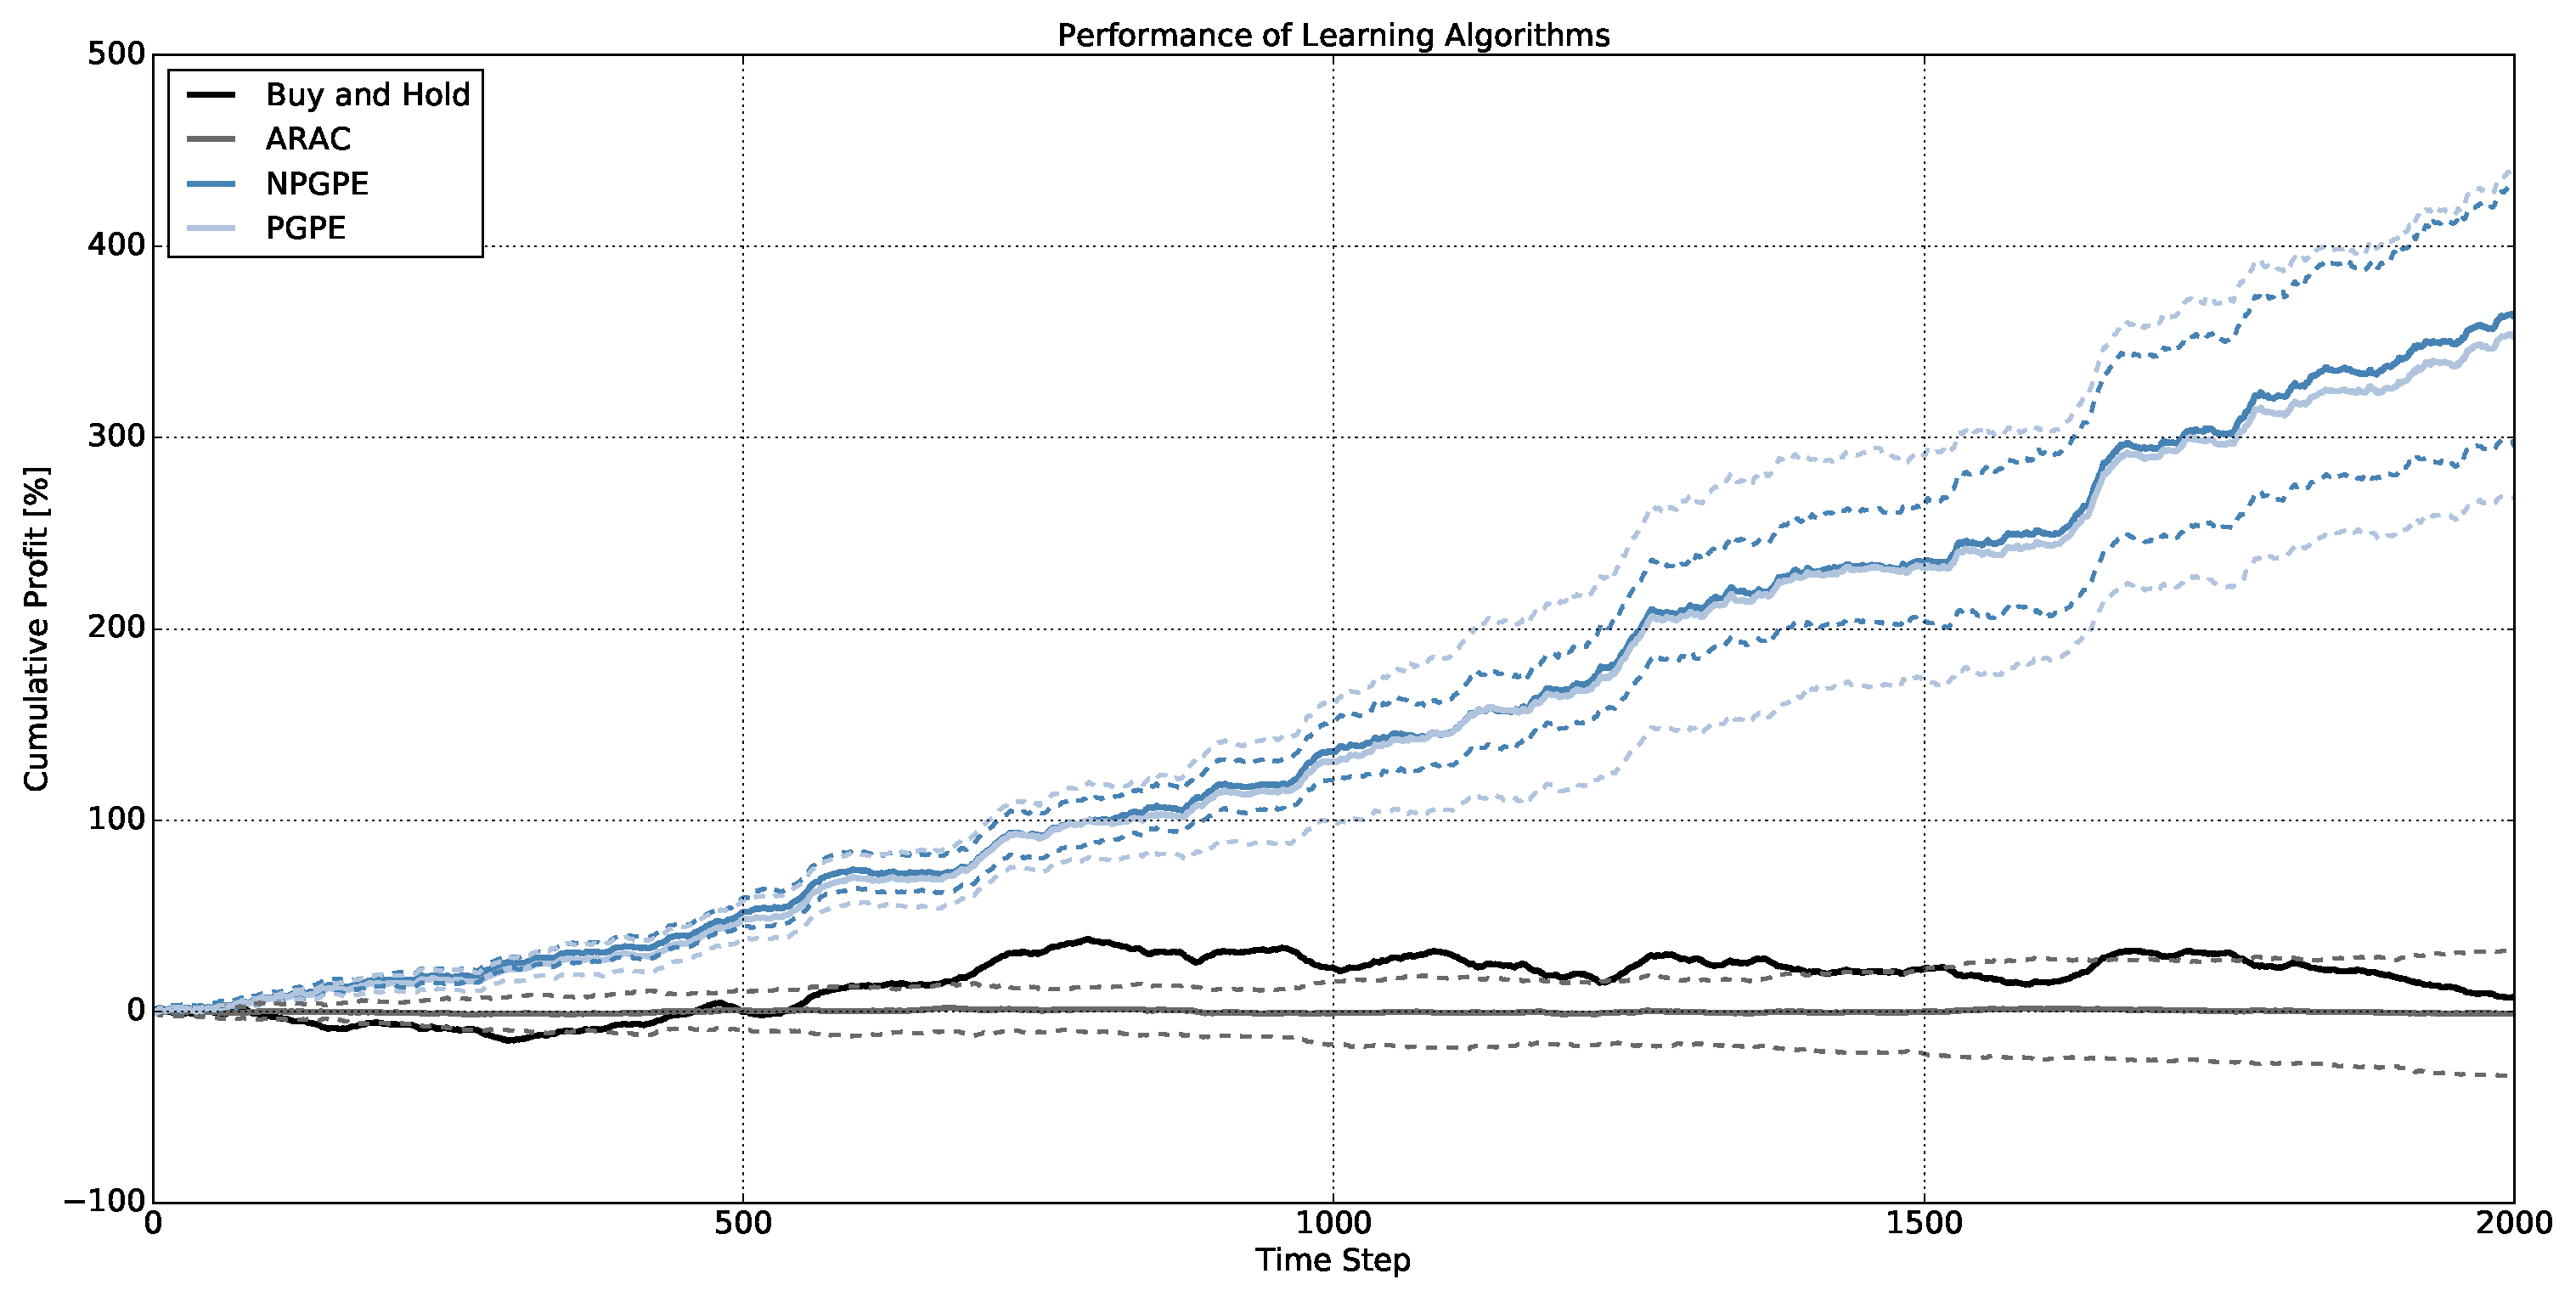
\includegraphics[height=6cm,width=0.8\textwidth]{Images/6_1_single_synthetic_neutral_performance}
%\end{figure}
%\end{frame}
%
%\begin{frame}[c]{Synthetic Asset: Impact of Transaction Costs}
%\begin{figure}[t!]
%	\centering
%	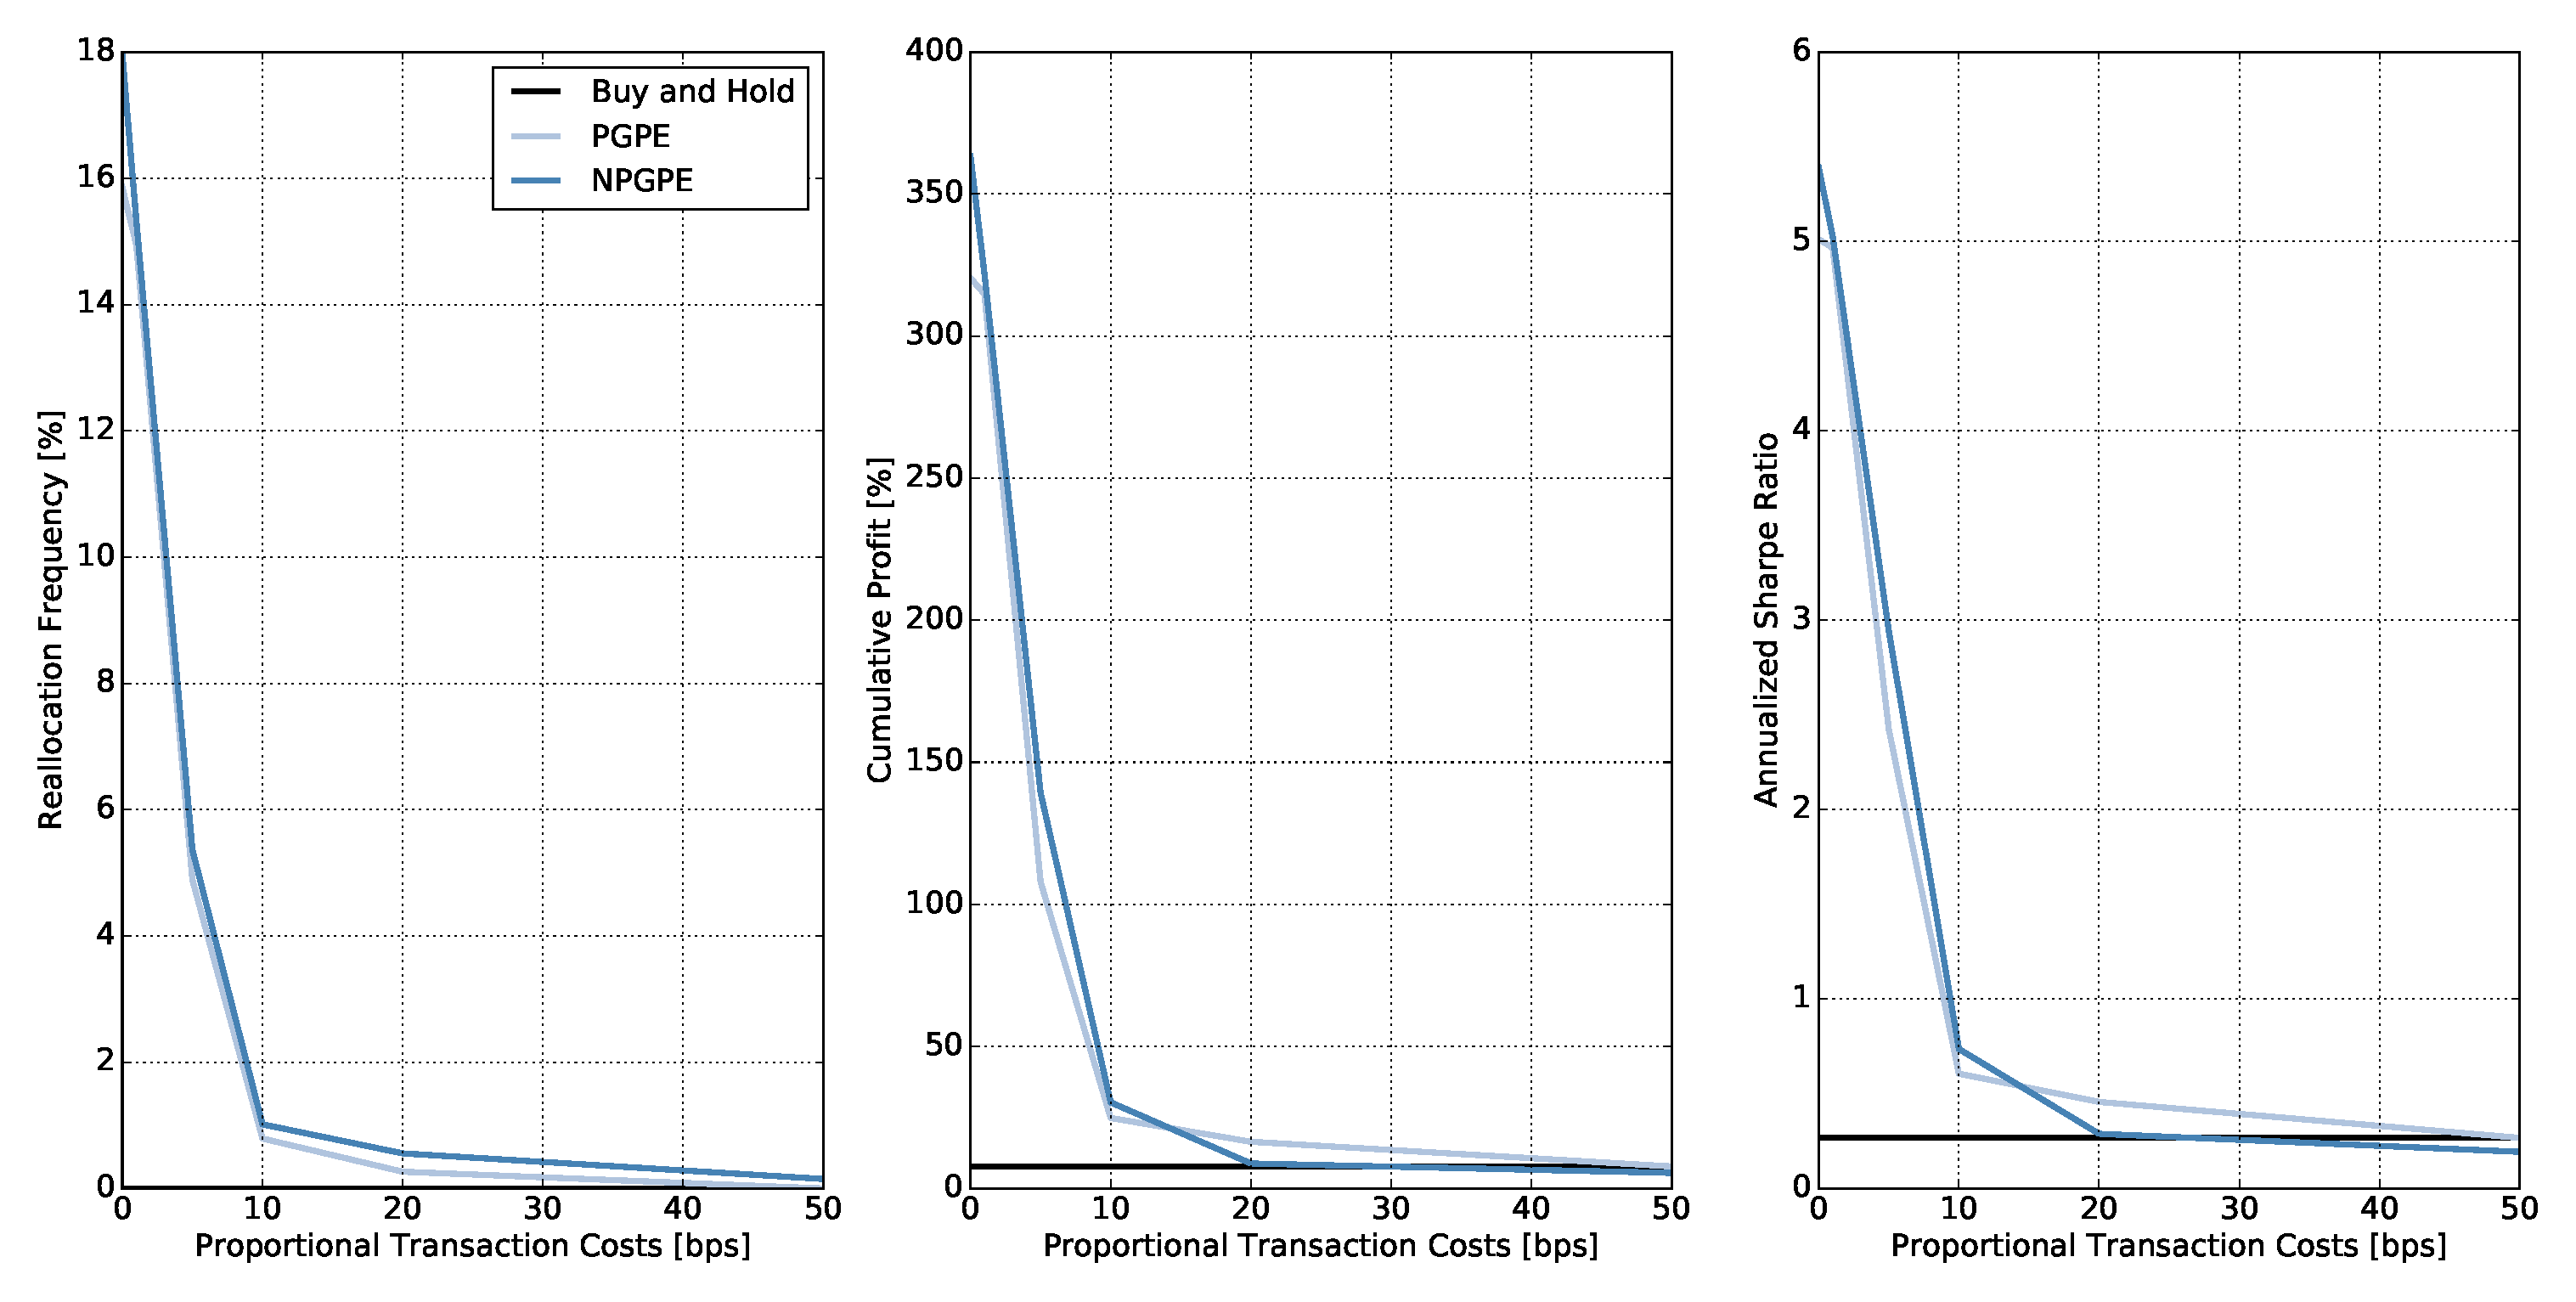
\includegraphics[height=3cm,width=0.8\textwidth]{Images/6_2_impact_transaction_costs}
%\end{figure}
%\begin{figure}[t!]
%	\centering
%	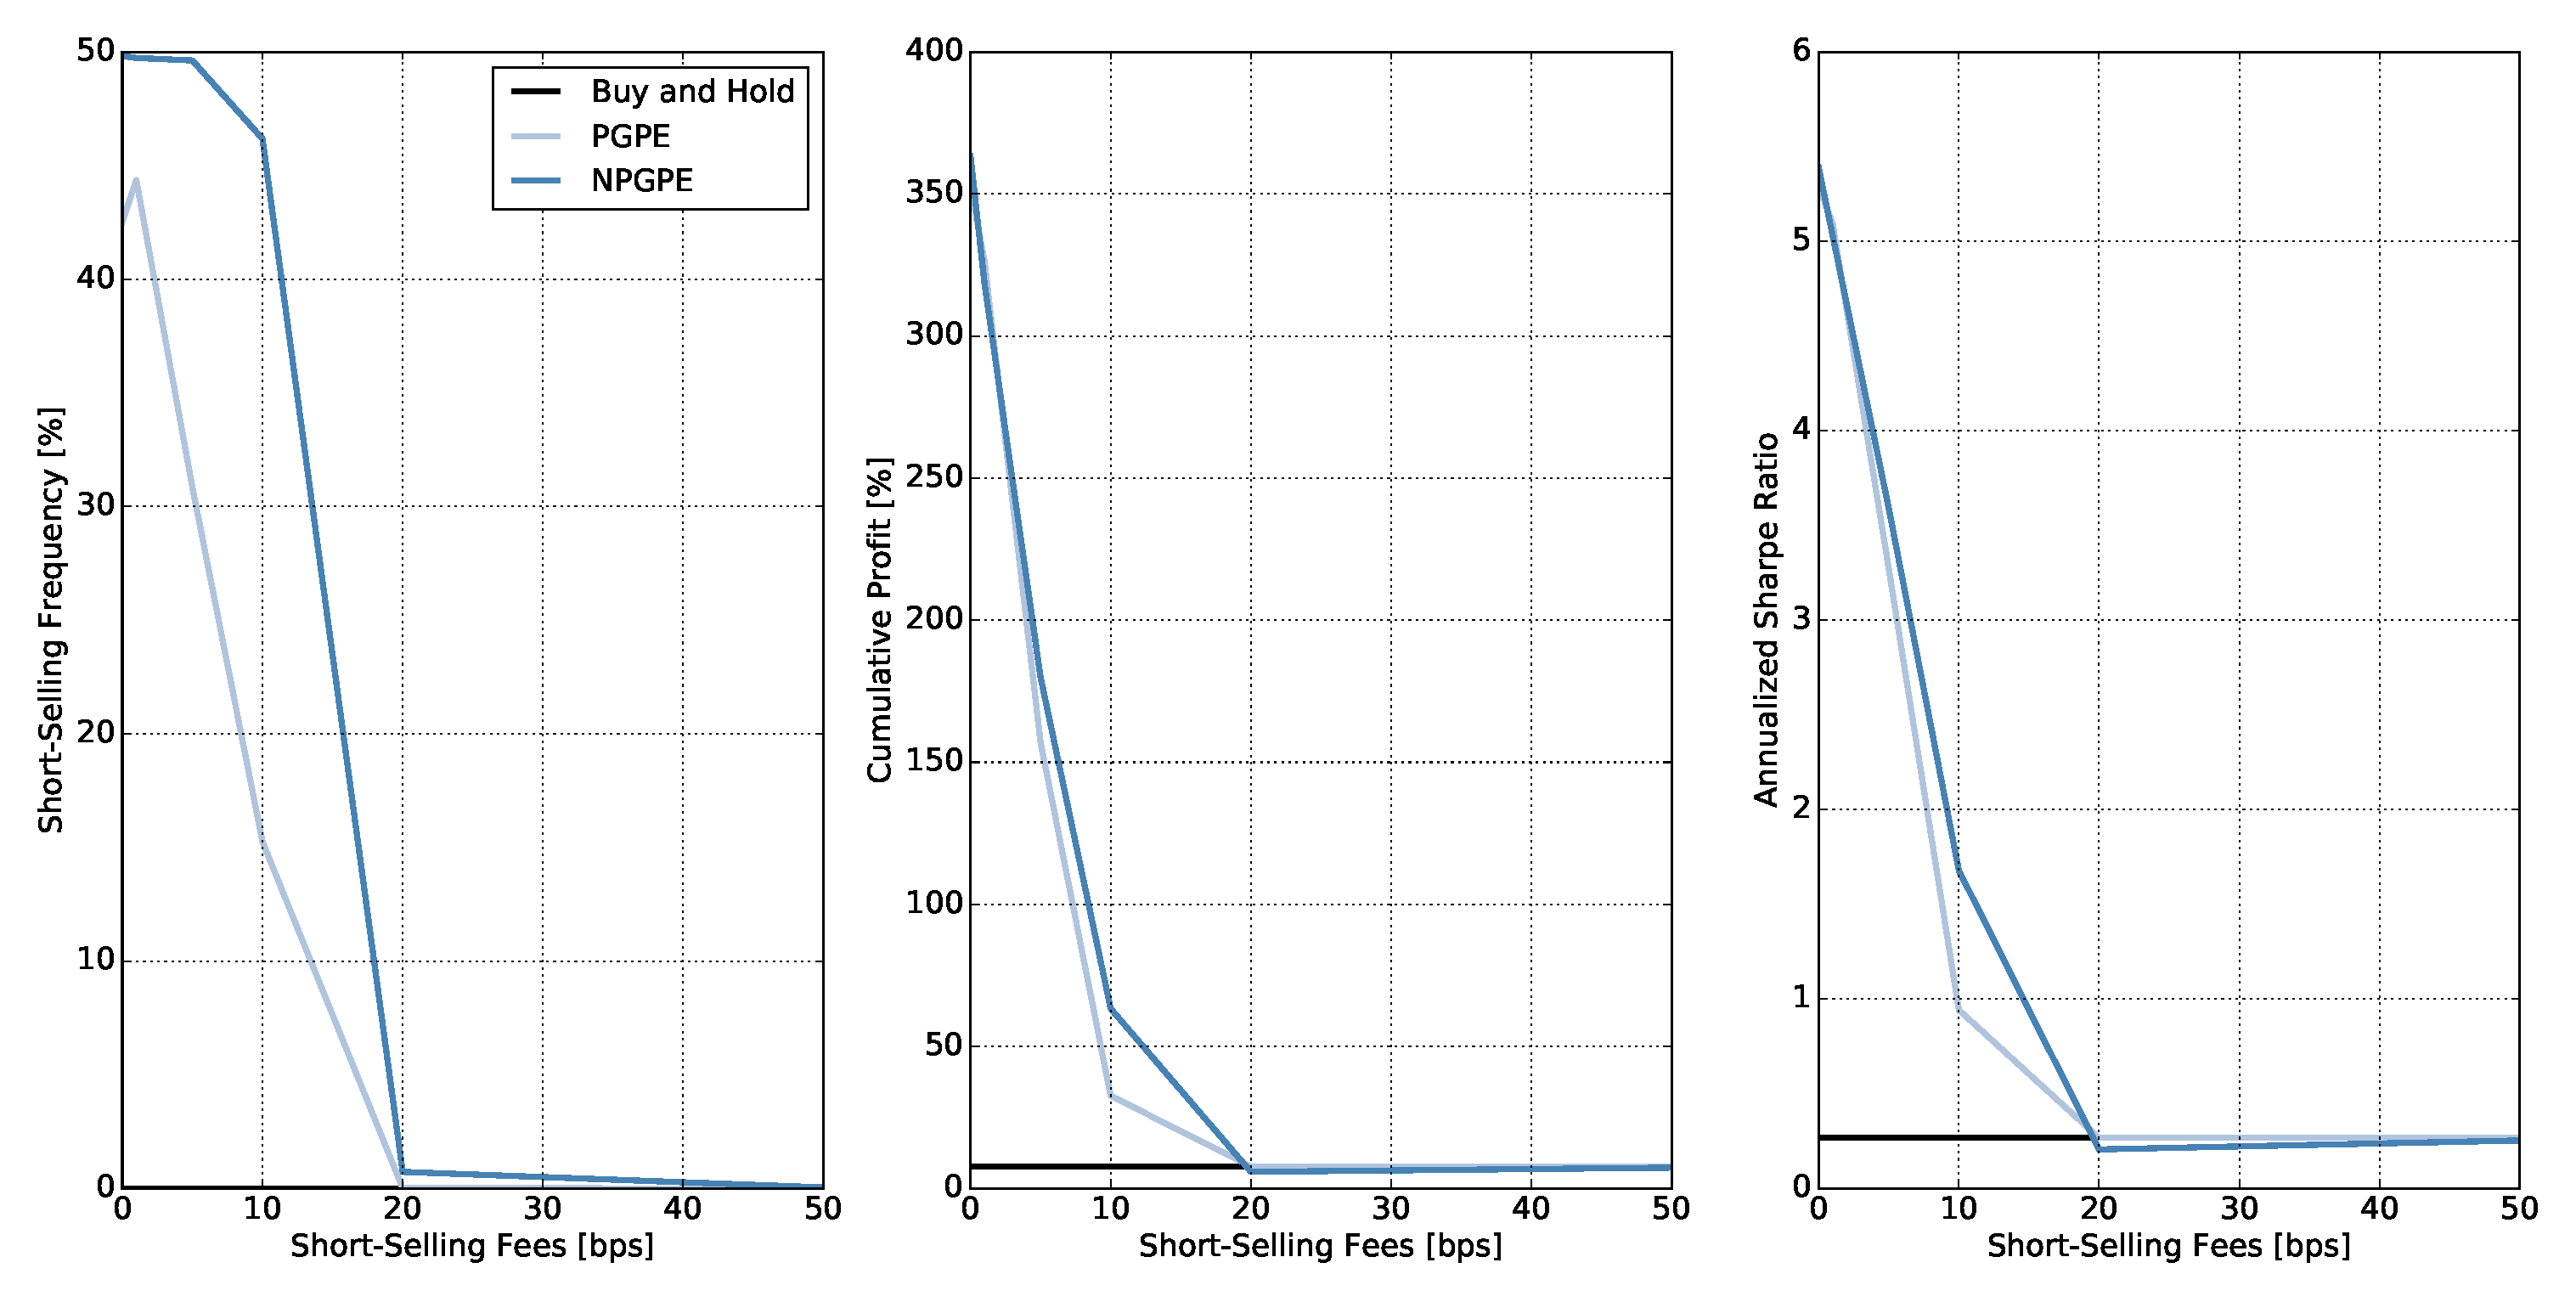
\includegraphics[height=3cm,width=0.8\textwidth]{Images/6_3_impact_short_selling_fees}
%\end{figure}
%\end{frame}
%
%\begin{frame}{Not So Fast}
%
%	\onslide<1->{
%	\begin{columns}
%	\begin{column}{0.6\textwidth}
%	   \begin{alertblock}{Insuccess on Historical Data}
%	   Successfully applying these RL algorithms to historical data is much more challenging
%	   \begin{enumerate}
%	   		\item Fail to converge
%	   		\item The strategies learned are not profitable
%	   \end{enumerate}
%	   \end{alertblock}
%	\end{column}
%	\begin{column}{0.4\textwidth}
%	    \begin{center}
%	     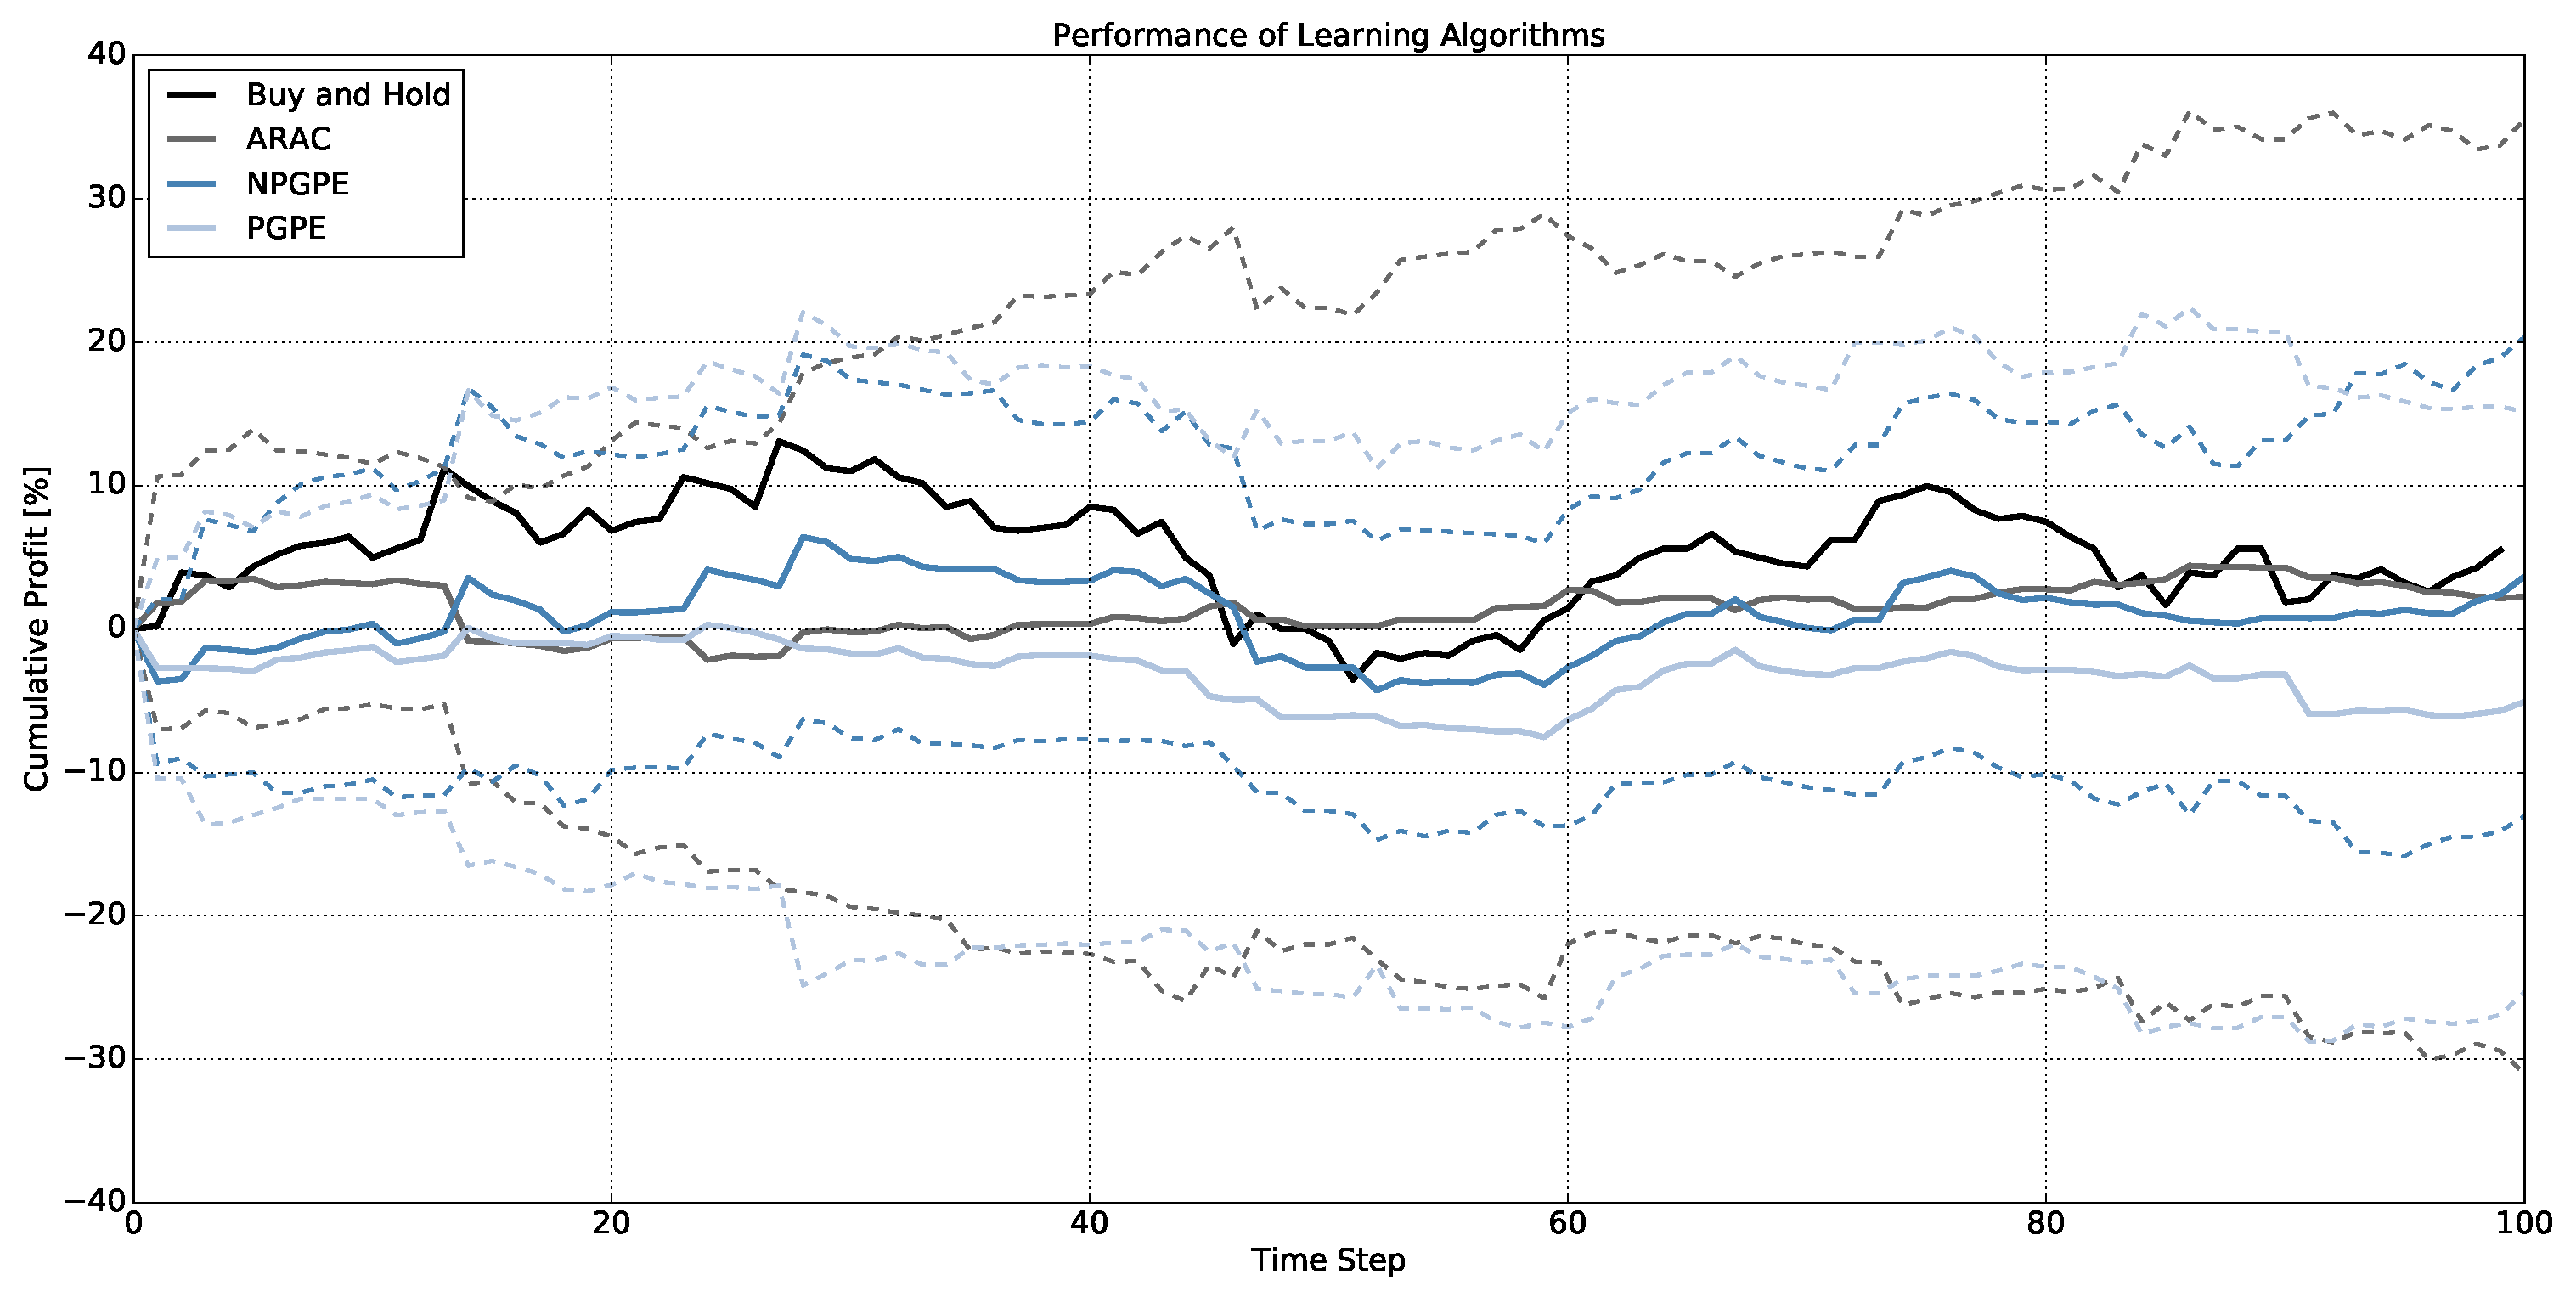
\includegraphics[width=1\textwidth]{Images/8_9_single_hist_neutral_performance}
%	     \end{center}
%	\end{column}
%	\end{columns}
%	}
%	
%	\onslide<2->{	
%	\begin{block}{Possible Explanations}
%		\begin{enumerate}
%			\item<2-> \textbf{Low signal-to-noise ratio}: extremely difficult to find tradable patterns in markets
%			\item<3-> \textbf{Quality of data}: unlikely to find patterns in daily prices of liquid stocks
%			\item<4-> \textbf{Weak features}: parametric policy must be powerful enough to capture the signal
%			\item<5-> \textbf{Non-stationarity of financial time-series}: a signal needs to be persistent
%		\end{enumerate}
%	\end{block}
%	}

